\begin{figure}[t]
\centering
\begin{subfigure}{0.5\linewidth}
\centering
\raisebox{1.05cm}{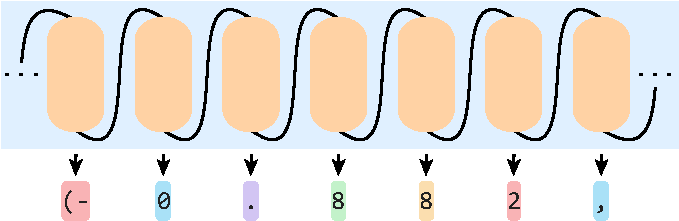
\includegraphics[width=\linewidth]{figures/diagram/not_numeric_head.pdf}}
\caption{Discretized numerics}
\label{fig:not_numeric_head}
\end{subfigure}
\hspace{1cm}
\begin{subfigure}{0.2350\linewidth}
\centering
\vspace{0.1cm}
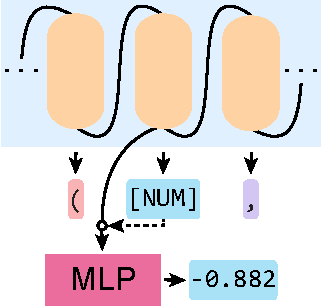
\includegraphics[width=\linewidth]{figures/diagram/numeric_head_diagram.pdf}
\caption{Continuous numerics}
\label{fig:numeric_head}
\end{subfigure}
\caption{\textbf{Numeric Head.} (\cref{ssec:numeric_head})
Rather than producing digits as discrete tokens (a), we train our model to generate a [NUM] token when a number should be produced.
The [NUM] token is used as a mask to signal the embedding should instead be passed through the numeric head, preserving the gradient (b).
}
\end{figure}